\newpage
\newgeometry{left=1.5cm, right=1.5cm, top=0.8cm, bottom=1cm}
\begin{figure}[p]
  \thispagestyle{empty} % Suppress the page number on this page
  \centering
  \captionsetup{justification=centering, labelfont=bf}
    \parbox{\textwidth}{\centering \Huge P0 derived Network - Leiden\vspace{0.5cm} } % 
    \label{fig:N_I:tum_P0}
    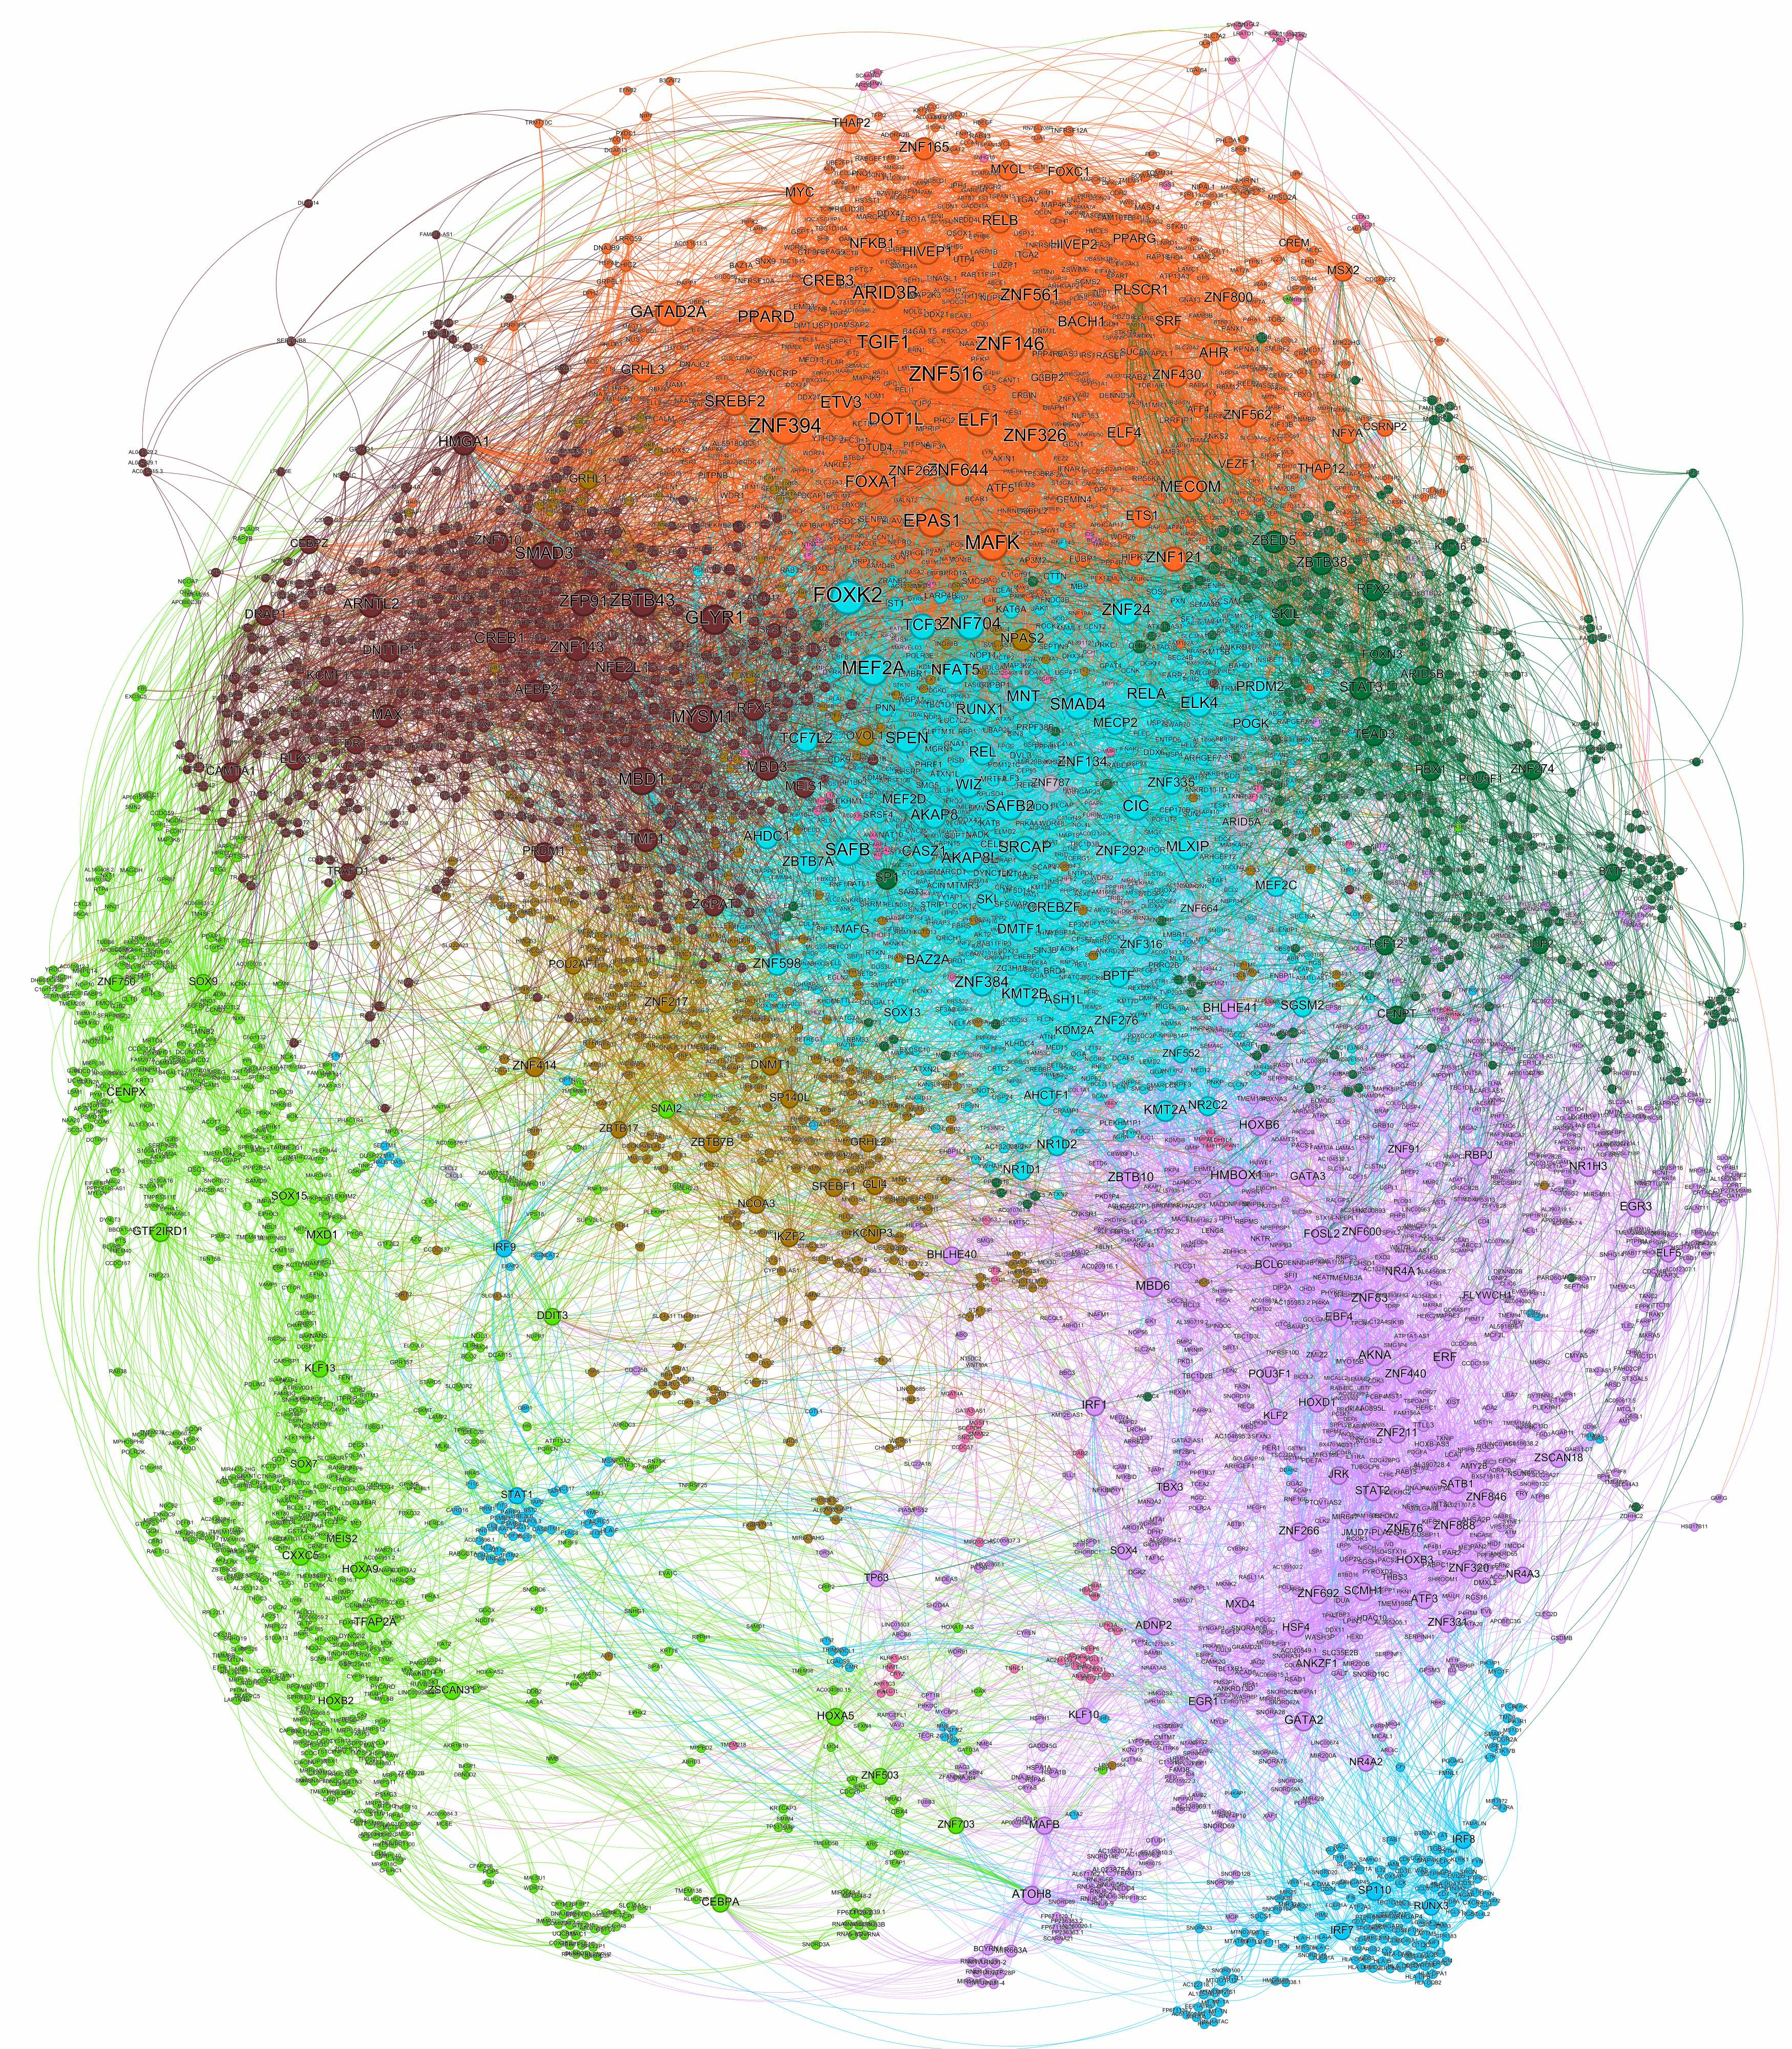
\includegraphics[width=0.9\paperwidth,keepaspectratio]{Sections/Network_pages/images/p0_std_4K_50TF_lowRes.jpg} % Full-page image
    \parbox{0.8\textwidth}{\centering Network created from using the 4000 most varied genes in the P0 dataset, no weight modifier, minimum degree of 3 for standard genes and 50 for TF.}
\end{figure}
\restoregeometry
\newpage
